\documentclass[class=article, crop=false]{standalone}
\usepackage[utf8]{inputenc}
\usepackage{graphicx}
\renewcommand{\baselinestretch}{1.5} 
\usepackage{wrapfig}
\usepackage{subcaption}
\usepackage{caption}
\usepackage{float}
\usepackage{xcolor}
\usepackage{amsmath}
\usepackage{blindtext}
\usepackage{import}
% \usepackage[backend=biber, style=numeric, citestyle=nature, doi=false, isbn=false, url=false, eprint=false]{biblatex} %Imports biblatex package, Comment out main doc
% \addbibresource{refs.bib} %Import the bibliography file, Comment out main doc

\begin{document} 
\label{section:Quad}

\section{Introduction}

Because of deuterium's ($^2$H) nuclear spin (I=1) being larger than 1/2 it possesses an electric quadrupolar magnetic moment (Q$_{\text{deuteron}}=$ 0.286 fm$^2$) \cite{Stone2015NuclearData}. This not only shortens the the relaxation times of $^2$H, it also introduces a frequency doublet which is similar to J-coupling or dipolar interactions. The frequency magnitude of the separation is dependent on the effect of ordering on the time-averaged direction of the local electric field gradient with respect to the magnetic field\cite{Seelig1977DeuteriumMembranes, Eliav2016MultipleMRS}. When performing MRSI each voxel will contain information from multiple different tissue/water compartments which can therefore complicate spectral appearance due to the superposition of ordered (anisotropic) and disordered (isotropic), and therefore the superposition is different frequency separations. The low available MR signal due to the low $^2$H natural abundance (0.015\%) means that quite often studies looking into this quantum effect are performed at high field \cite{Gursan2022ResidualMuscle} and\cite{Ooms2015DoubleTissue}/or\cite{Damion2022DoubleLoading} increasing $^2$H abundances using D$_2$0. In order to keep the spectral behaviour simple and negate the effects from isotropic compartments double quantum filtering (DQF) can be used\cite{Sharf1995DetectionNMR-Spectroscopy, Perea20072HDisc}, however this greatly reduces the available SNR. 

The combinations of spin operators ($I_x, I_y$ and $I_z$) can be represented as spherical operator tensors ($T_{l,p}$), where $l$ is the rank and $p$ is the coherence of the tensor, noting that $|p| \le l$. Since $^2$H is $I=1$ no rank greater than two can be reached, which means the only multiple quantum (MQ) that can be achieved is the double quantum coherences represented by the $T_{2,\pm2}$ tensors, this only arises from anisotropic medium. DQF suppresses the single quantum coherences ($T_{1,\pm1}$) leaving only signal from the anisotropic regions from the $T_{2,\pm2}$. By using DQF to measure measure the anisotropy of tissues and fluids in the body such as intervertebral disc tissue \cite{Ooms2015DoubleTissue}, brain water\cite{Assaf1997InSpectroscopy} and elastin\cite{Sun2010InvestigationNMR} reveals a lot about the presence of diseases such as degenerative disc disease\cite{Ooms2015DoubleTissue}.

\subsection{Aims}

Healthy human participants ingested a D$_2$O and H$_2$O solution to increase their $^2$H abundance. The dependency of quadrupolar splitting frequency to angular orientation of skeletal muscle in a magnetic field was then measured, using CSI data in the forearm and the calf at 3T using an in-house built saddle coil and helmholtz coil. Bulk and CSI, DQF data was also obtained with varying $\tau$ values and different angles. 

\section{Theory}
\subsection{Quadrupolar Splitting}

The quadrupolar moment interacts with the local electric field gradients (EFG) which can be represented as a combination of up to six electric potential tensor elements, these are then simplified to three principal axis elements ($V_{xx}, V_{yy}$ and $V_{zz}$). By definition the sum of these elements is 0, as the EFG is a traceless tensor. $V_{zz}$ is defined as the largest element and is usually specified as the EFG at the quadrupolar nucleus ($V_{zz} = e\cdot q$)\cite{Elliott2021WhatMedia}. The ratio of the difference between $V_{xx}$ and $V_{yy}$ to $V_{zz}$ is referred to as the asymmetry parameter ($\eta$).
\begin{equation}
    \eta = \frac{V_{xx}-V_{yy}}{V_{zz}}
\end{equation}
By considering the time-independent Hamiltonian ($H_Q$) of this interaction it is possible to find a mathematical generalised form.
\begin{equation}
    H_Q = \frac{eQ}{4I(2I-1)}[V_0(3I^2_z-\boldsymbol{I}^2) + V_{\pm1}(I_{\mp}I_z+I_zI_\mp)+V_{\pm2}I^2_\mp]
\end{equation}
$V_0$, $V_{\pm1}$ and $V_{\pm2}$ are the three principal axis elements combined to create new elements, which are complex, that better represent the total EFG. When considering the rotational transformation from the molecule's fixed reference frame to the laboratory fixed reference frame\cite{Seelig1977DeuteriumMembranes}, along with an assumed value of $\eta$=0 (uniaxiality), the total Hamiltonian simplifies for deuterium ($I$ = 1) \cite{Sharf1995DetectionNMR-Spectroscopy}. The form of this equation, now using its simplified principal axis elements is:
\begin{equation}
    H = -g\beta_N\boldsymbol{I}\cdot\boldsymbol{H_0} + \frac{eQ(3\cos^2(\theta)-1)}{8}V_{zz}(3I_z^2-\boldsymbol{I}^2)
\end{equation}
where $g$ is the g-factor, $\beta_N$ is the nuclear magneton, Q is the (scalar) quadrupole moment, $\boldsymbol{H_0}$ is the magnetic field, $e$ is the charge of an electron, $I$ is the nuclear spin (of deuterium) and $\theta$ is the angle between the electric potential and the magnetic field. Now that a simplified total Hamiltonian is found the perturbed energy levels can be calculated, which will have an associated energy difference and therefore a frequency difference.
\begin{equation}
    \nu_Q(\theta) = \frac{3}{2}\left(\frac{e^2qQ}{h}\right)\left(\frac{3\cos^2(\theta)-1}{2}\right)
    \label{eqn:Quad:Angle}
\end{equation}
where the RQC in this case is given in the first part of the above equation.
\begin{equation}
    \omega_Q/2\pi = \frac{3}{2}\left(\frac{e^2qQ}{h}\right)
    \label{eqn:Quad:RQC}
\end{equation}

The above derivation shows that as a result of the quadrupolar magnetic moment interacting with the EFG a splitting is observed that is caused by perturbed energy levels. The frequency magnitude of this splitting effect is quantifiable and depends only on the orientation of the deuterated sample to the applied magnetic field (equation \ref{eqn:Quad:Angle}. In an isotropic structure such as the brain this splitting effect is not visible due to averaging resulting from molecular motion. In an anisotropic media such as the skeletal muscle fibres in the calf, the quadrupolar splitting is at a maximum and equal to the RQC value when the deuterated sample is orientated with the magnetic field ($\theta = 0^\circ$). The splitting effect can also be nulled ($\nu_Q = 0$) if the sample is orientated to the magnetic field at the magic angle $\theta = 54.74^\circ$ ($\cos^2\theta=1/3$).

This detected signal from the DQF signal is related to a second rank tensor arising from the EFG, which can only be formed in anisotropic media/phases. Therefore it is possible to measure the RSC constant from these NMR spectra which provides information on the anisotropy of the media investigated. This technique is applied by manipulating the pulse sequence with alternating $\pi/2$ and $\pi$ RF pulses. 

\subsection{Quantum Filtering}

\begin{figure}
    \centering
    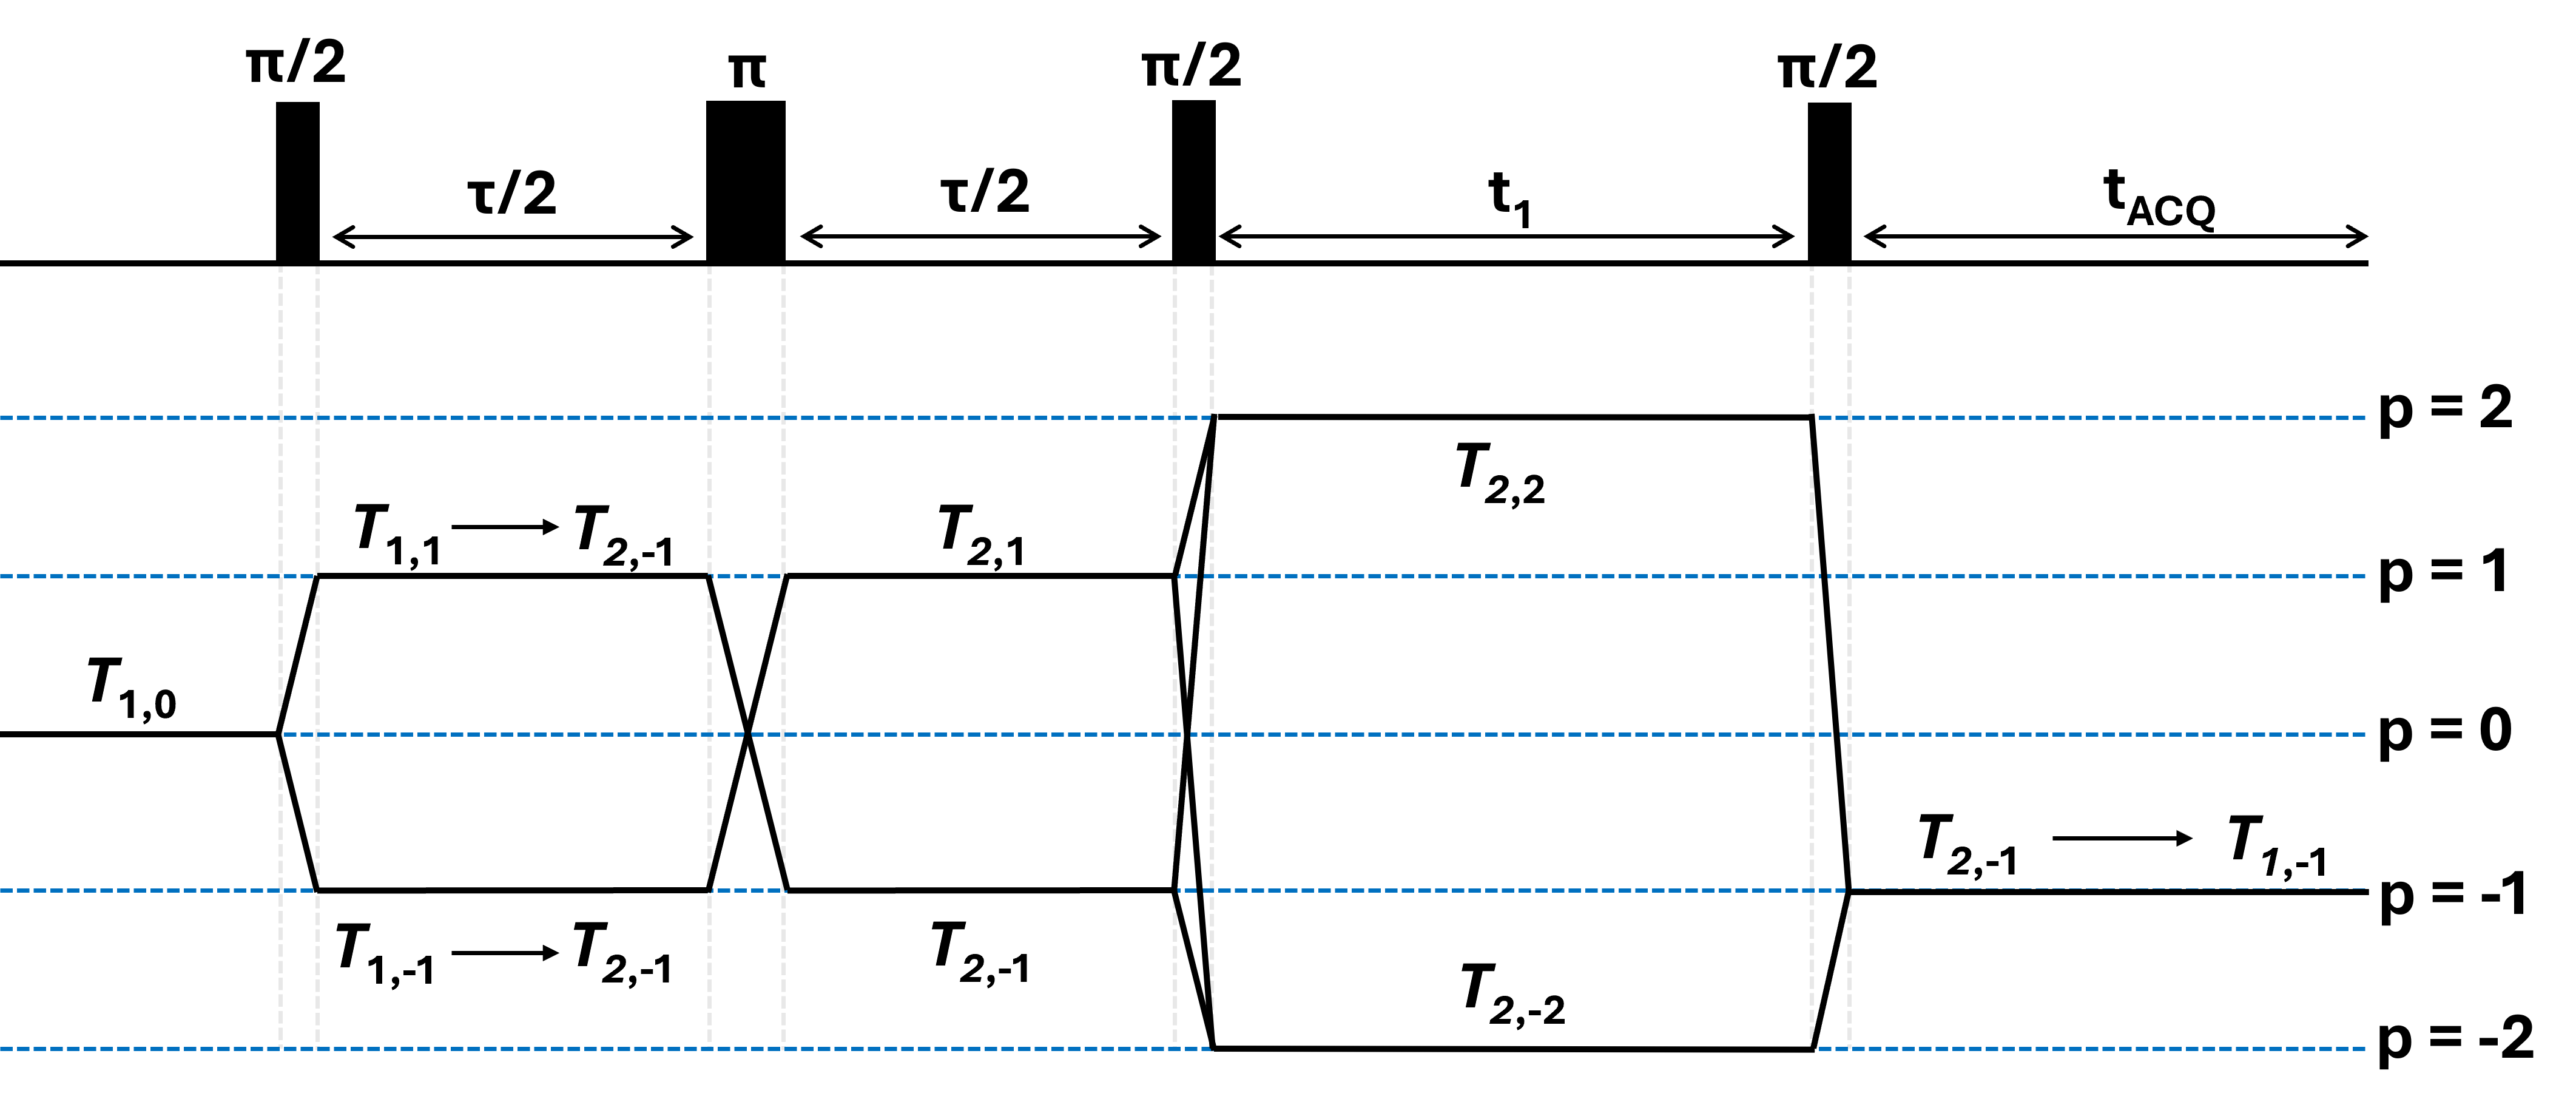
\includegraphics[width=1\textwidth]{Figures/Quad/DQF_Coherence.png}
    \caption{The coherence pathway and the RF pulse sequence during a DQF acquisition. Noting that the tensor $T_{l,p}$ includes information on the rank ($l$) and on the coherence ($p$), which is indicated on the right side.}
    \label{fig:Quad:Coherence}
\end{figure}

A pulse sequence that can be used to suppress the single quantum coherence and the obtain the double quantum coherence is shown below\cite{Sharf1995DetectionNMR-Spectroscopy}, where the pulse angles and the wait times are shown below. It is important that the correct phase cycling is used\cite{Bodenhausen1984SelectionExperiments}, the following transmit phase cycling is used here 0$^\circ$, 90$^\circ$, 180$^\circ$ and 270$^\circ$ and the following receive phase 0$^\circ$, 270$^\circ$, 180$^\circ$ and 90$^\circ$. 

\begin{equation}
    \pi/2-\tau/2-\pi-\tau/2-\pi/2-t_1-\pi/2-t_2 \textrm{ (Acquisition)}
    \label{eqn:Quad:Pulse}
\end{equation}

The $t_1$ period suppresses the single coherence's and the last pulse refocuses the double coherence's together so that the signal is detectable. The obtained FID appears as two anti-phase Lorentzian lineshapes with a separation frequency, if the separation is small this behaviour can be difficult to identify as the curves overlap. The amplitude of the DQF FID follows a damped sinusoid.

\begin{equation}
    A\sin(2\pi\nu_q\tau)\exp(-2\tau/T_2)
    \label{eqn:Quad:Amplitude}
\end{equation}

Where $T_2$ is a transverse relaxation, $A$ is an amplitude coefficient, $\nu_q$ is the splitting frequency and $\tau$ is known as the creation time and is the time between the first two $\pi/2$ pulses. This assumes perfect flip angles and that the signal is on-resonance. The coherence transfer pathway with the changing tensors can be seen in Figure \ref{fig:Quad:Coherence}.

% Example DQF Spectra

\section{Scanning}

Measurements for this work was obtained in two separate investigations that both used the ingestion of D$_2$O and H$_2$O solution to increase $^2$H. Different loading routines were implemented in each investigation and both took place at different times. Each part of the first investigation had a different number of participants, while the second investigation had three participants for each part (two of which also took part in the previous investigation). Due to the different loading routines being different the overall $^2$H abundances will be different, the exact SNR is not important to either investigation as long as it was possible to obtain data in a reasonable time frame. The loading routine for the first investigation was the same that was used in chapter \ref{section:D2O}, and the loading routine for the second investigation was the same as in chapter \ref{section:Lipid}.

All data was obtained using a Philips 3T Achieva scanner, all $^1$H anatomical scans were performed using the built-in body coil using a 3D GE scan. $^2$H data was obtained using in-house built coils details of which can be found in chapter \ref{section:Theory:Coils}. 

\subsection{Study One}
\subsubsection{Quadrupolar Splitting}
\label{Chap:Quad:1:Split}

After the initial D$_2$O loading period was completed and the participants $^2$H enrichment had reached a steady state level. The left calves of two participants (A and B) were scanned using the in-house built $^2$H saddle coil. 3D chemical shift images were obtained with 10 mm isotropic voxels, NSA = 2, samples = 256, TE = 6.2 ms, TR = 500 ms, BW = 750 Hz, FOV = 120x120x60 mm$^3$, the CSI was originally obtained to look at the overall spread of $^2$H enrichment in skeletal muscle (see Chapter \ref{section:D2O}). However quadrupolar splitting was observed across the calf (most notably in the tibialis anterior muscle). This was used as motivation to investigate the effect of quadrupolar splitting in skeletal muscle.

The participants were therefore scanned again using the in-house built Helmholtz coil designed to scan the forearm. The left forearms of A and B were scanned as this allowed us to easily bend the arm in the coil at different angles with respect to the B$_0$ field of the magnet, which allows us to change $\theta$ in equation \ref{eqn:Quad:Angle}. A $^2$H 3D CSI with 10x10x15 mm$^3$ voxels, NSA = 2, 256 samples, TE = 6.4 ms, TR = 363 ms, BW = 750 Hz and FOV = 120x120x60 mm$^3$ is acquired for a range of different arm angles was acquired. During scanning, for each angle, participants were lay in a prone position with their left arm above their head. A 'straight' arm represented  0$^{\circ}$ angle respect to the B0 field, participant A was then scanned with angles of 0, 10, 20, 30 and 40$^{\circ}$ in one visit and 50, 60, 70, 80 and 90$^{\circ}$ in a second visit. Participant B was scanned with angles 0, 85, 30, 15, 45, 60, 75 and -10$^{\circ}$ in a single visit. 

The 3D CSI spectra for the forearm was analysed using MATLAB and started with zero-order phase correction and masked based on the maximum value from the spectra of a specific voxel being larger than 20\% of the maximum value of all spectra. Each voxel within the mask was then fit to two complex Lorentzian curves with equal amplitudes, phases and linewidths where the frequency splitting between the two peaks is determined from fitting. The spectra is also fit to three complex Lorentzian curves where the two 'outer' peaks have equal equal amplitudes, phases and linewidths similar to before except now there is a third central peak with different amplitude, phase and linewidth to the other peaks the frequency splitting is now the frequency difference between the 'outer' two peaks only. The fitting is performed by minimising the sum of the squared difference between the proposed fit and the phase-corrected signal, this was done using in-built MATLAB function fmincon. The best fit is determined by comparing the final minimised value returned from fitting, whichever combination of Lorentzian curves gave the lowest value is kept and outputted for that voxel. The frequency splittings are then averaged over the masked region to give a single frequency splitting. This process was repeated for each angle, with the angle values being obtained from the angulation of the imaging/spectroscpy FOV. All the splitting's were then fit to equation \ref{eqn:Quad:Angle}, where the total RQC is determined. This was repeated for participants A and B.

\subsubsection{Double Quantum Filtering}

Deuterium spectroscopy and chemical shift imaging (CSI) were performed on lower legs and forearms in four healthy human participants (A,B,C and D). $^2$H spectra were acquired from a 2 cm axial slice of the calf or forearm, by using hard pulses in combination with outer-volume saturation. DQF spectra were created by using the sequence in Figure \ref{fig:Quad:Coherence}, which produces an anti-phase spectrum whereby the quadrupolar doublet peaks acquire a relative phase of 180° (see Figure \ref{}). This relative phase means that the signal vanishes for any components if their splitting frequency is small. DQF spectra are phased to produce a symmetric line-shape (labelled as dispersion spectra in anti-phase in Figure \ref{}).  

DQF spectra were acquired for various values of $\tau$, (take from ISMRM figure 1) and TR = 1000 ms, TE = 0.58 ms, bandwidth = 3000 Hz, samples = 1024. The number of averages varied, depending on available signal, between 28 and 128. FID's were processed using Matlab scripts and spectra were fit to a maximum of three independent Lorentzian line shapes.

Deuterium 2D CSI data were also acquired from a single 2 cm axial slice, again using outer-volume suppression. 2D CSI data were acquired for the usual pulse-acquire sequence, and using the anti-phase DQF sequence with $\tau$ = 6.5 ms. The voxel volume was 10x10 mm$^2$, TR = 378 ms, TE = 3.9 ms, samples = 256 and bandwidth = 750 Hz. For the DQF CSI, 16 averages were acquired, whereas only 4 were needed for the pulse-acquire CSI.

\subsection{Study Two}
\subsubsection{Quadrupolar Splitting}

$^2$H 3D CSI data were acquired with 10x10x10 mm$^3$ voxels, FOV = 120x120x50 mm$^3$, TR =500 ms, TE = 6.2 ms, bandwidth = 750 Hz, samples = 256 and NSA = 2 in three healthy human participants (A,B and E). Images were acquired in each subject with the forearm at 10 different angles ($\approx$0 – 90$^\circ$) to the field. The protocol here was similar to what followed in the above section (chapter \ref{Chap:Quad:1:Split}). 

In order to ensure that the forearm was always in the centre of the field, that a large enough range of angles were covered and that each participant was as comfortable as they could be. Each participant was removed from the scanner in between each angle, which is why commonly scanning ran over two days. The protocol for each angle included $^1$H scout scan and GE anatomical, two bulk spectra and finally a 3D CSI. For angles larger than 45$^\circ$ the data had to be acquired sagittally as oppose to transverse.

Whilst the study is similar to what was done previously in chapter \ref{Chap:Quad:1:Split}, one of the major differences is in the analysis routine. % Angle Calculation

A zero-order phase correction was applied to all spectra, as well as de-noising through a Tucker decomposition\cite{Bader2007EfficientTensors} with a compression core matrix of [64,6,6,3] (spectral, followed by three spatial dimensions). A binarised mask with the same spatial resolution as the CSI is then constructed, following thresholding of 35\% of the maximum spectral signal (the mask was then filled using imfill). The OXSA-AMARES toolbox in Matlab was then used to fit three Lorentzian peaks to each masked voxel, centre peak with an outside doublet due to quadrupolar splitting (each peak in the doublet has the same linewidth and amplitude, all peaks are fit with the same phase). The initial estimate of the seperation of the doublet varied depending on the angle of the arm in the scanner. The separation of the doublet was converted from ppm to Hz and then the values, along with the arm angle, was fit to equation \ref{eqn:Quad:Angle}.

\subsubsection{Double Quantum Filtering}

%Re-Write

DQF spectra were acquired for various values of the creation time, $\tau$, (see Figure \ref{fig:Quad:Coherence}) and TR/TE=1000/0.58 ms, sampling bandwidth 3000 Hz, 1024 samples. The number of averages varied, depending on available signal, between 28 and 128. FIDs were processed using Matlab scripts and spectra were fitted to a maximum of three independent Lorentzian line shapes.

Deuterium CSI data were also acquired from a single 2 cm axial slice, again using outer-volume suppression. CSI data were acquired for the usual pulse-acquire sequence, and using the anti-phase DQF sequence with $\tau$=6.5 ms. The in-plane resolution was 10x10 mm2,  TR/TE=378/3.9 ms, 256 samples were acquired at a bandwidth of 750 Hz. For the DQF CSI, 16 averages were acquired, whereas only 4 were needed for the pulse-acquire CSI.

% Talk about fitting and OXSA

\section{Results}

\subsection{Quadrupolar Splitting}

\begin{figure}
    \centering
    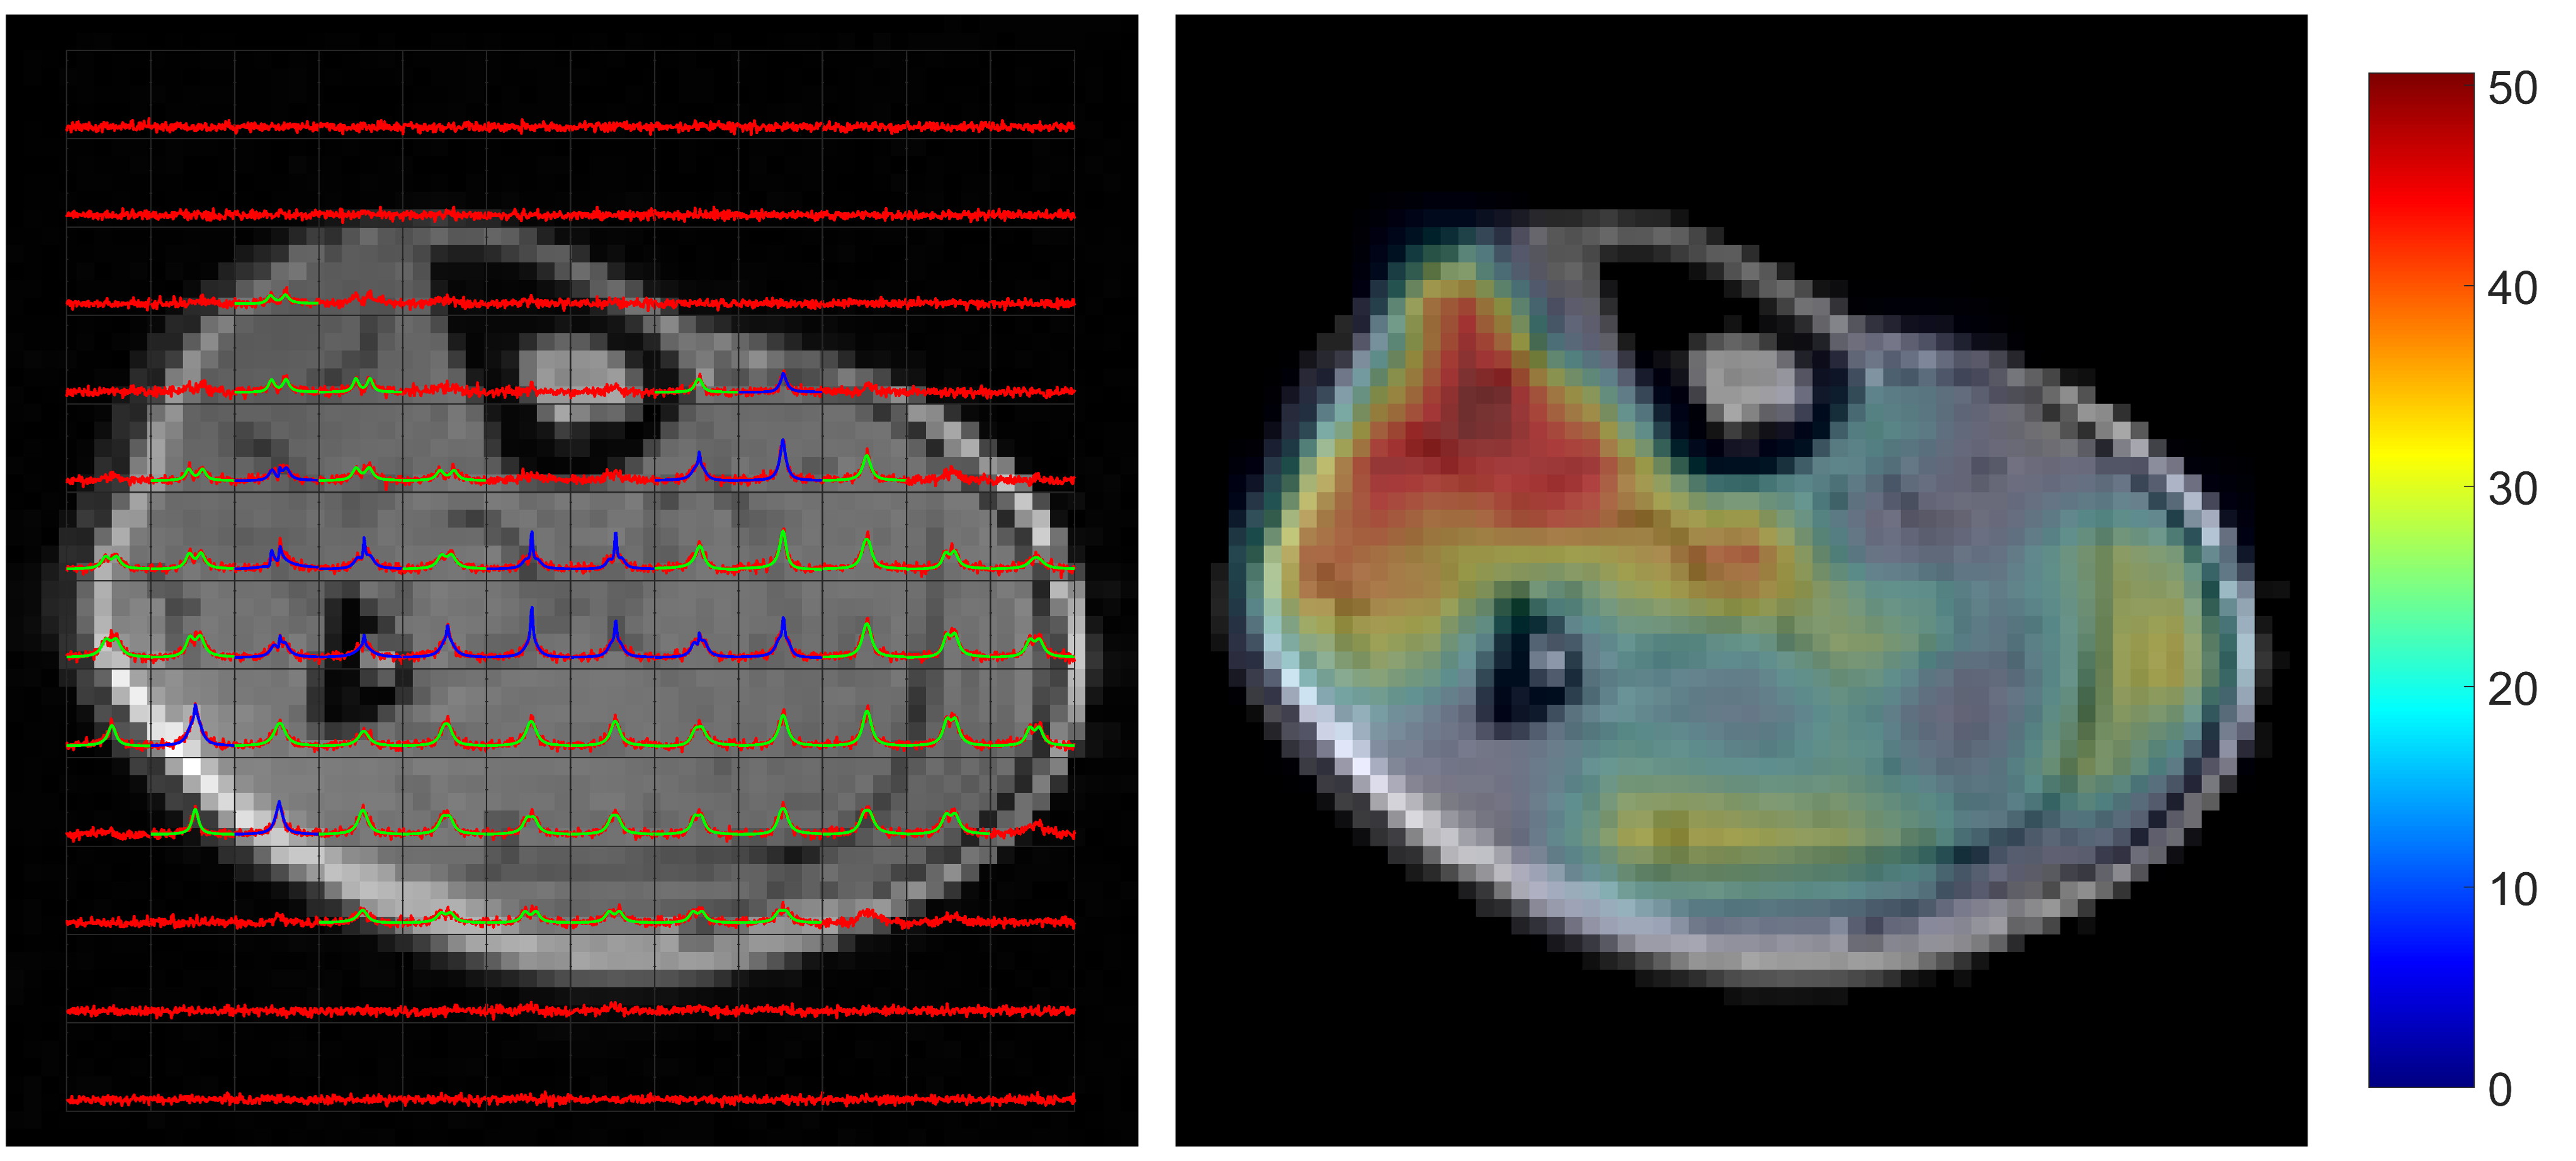
\includegraphics[width=1\textwidth]{Figures/Quad/Calf_A.png}
    \caption{Left: CSI spectra (red) overlayed onto a $^1$H GE image from participant A's left calf of a single slice, with fits of two Lorentzian peaks (green) and three Lorentzian peaks (blue). Right: Interpolated map of quadrupolar frequency splitting's overlayed onto the same $^1$H GE image from participant A's left calf. }
    \label{fig:D2O:Calf_A}
\end{figure}

\begin{figure}
    \centering
    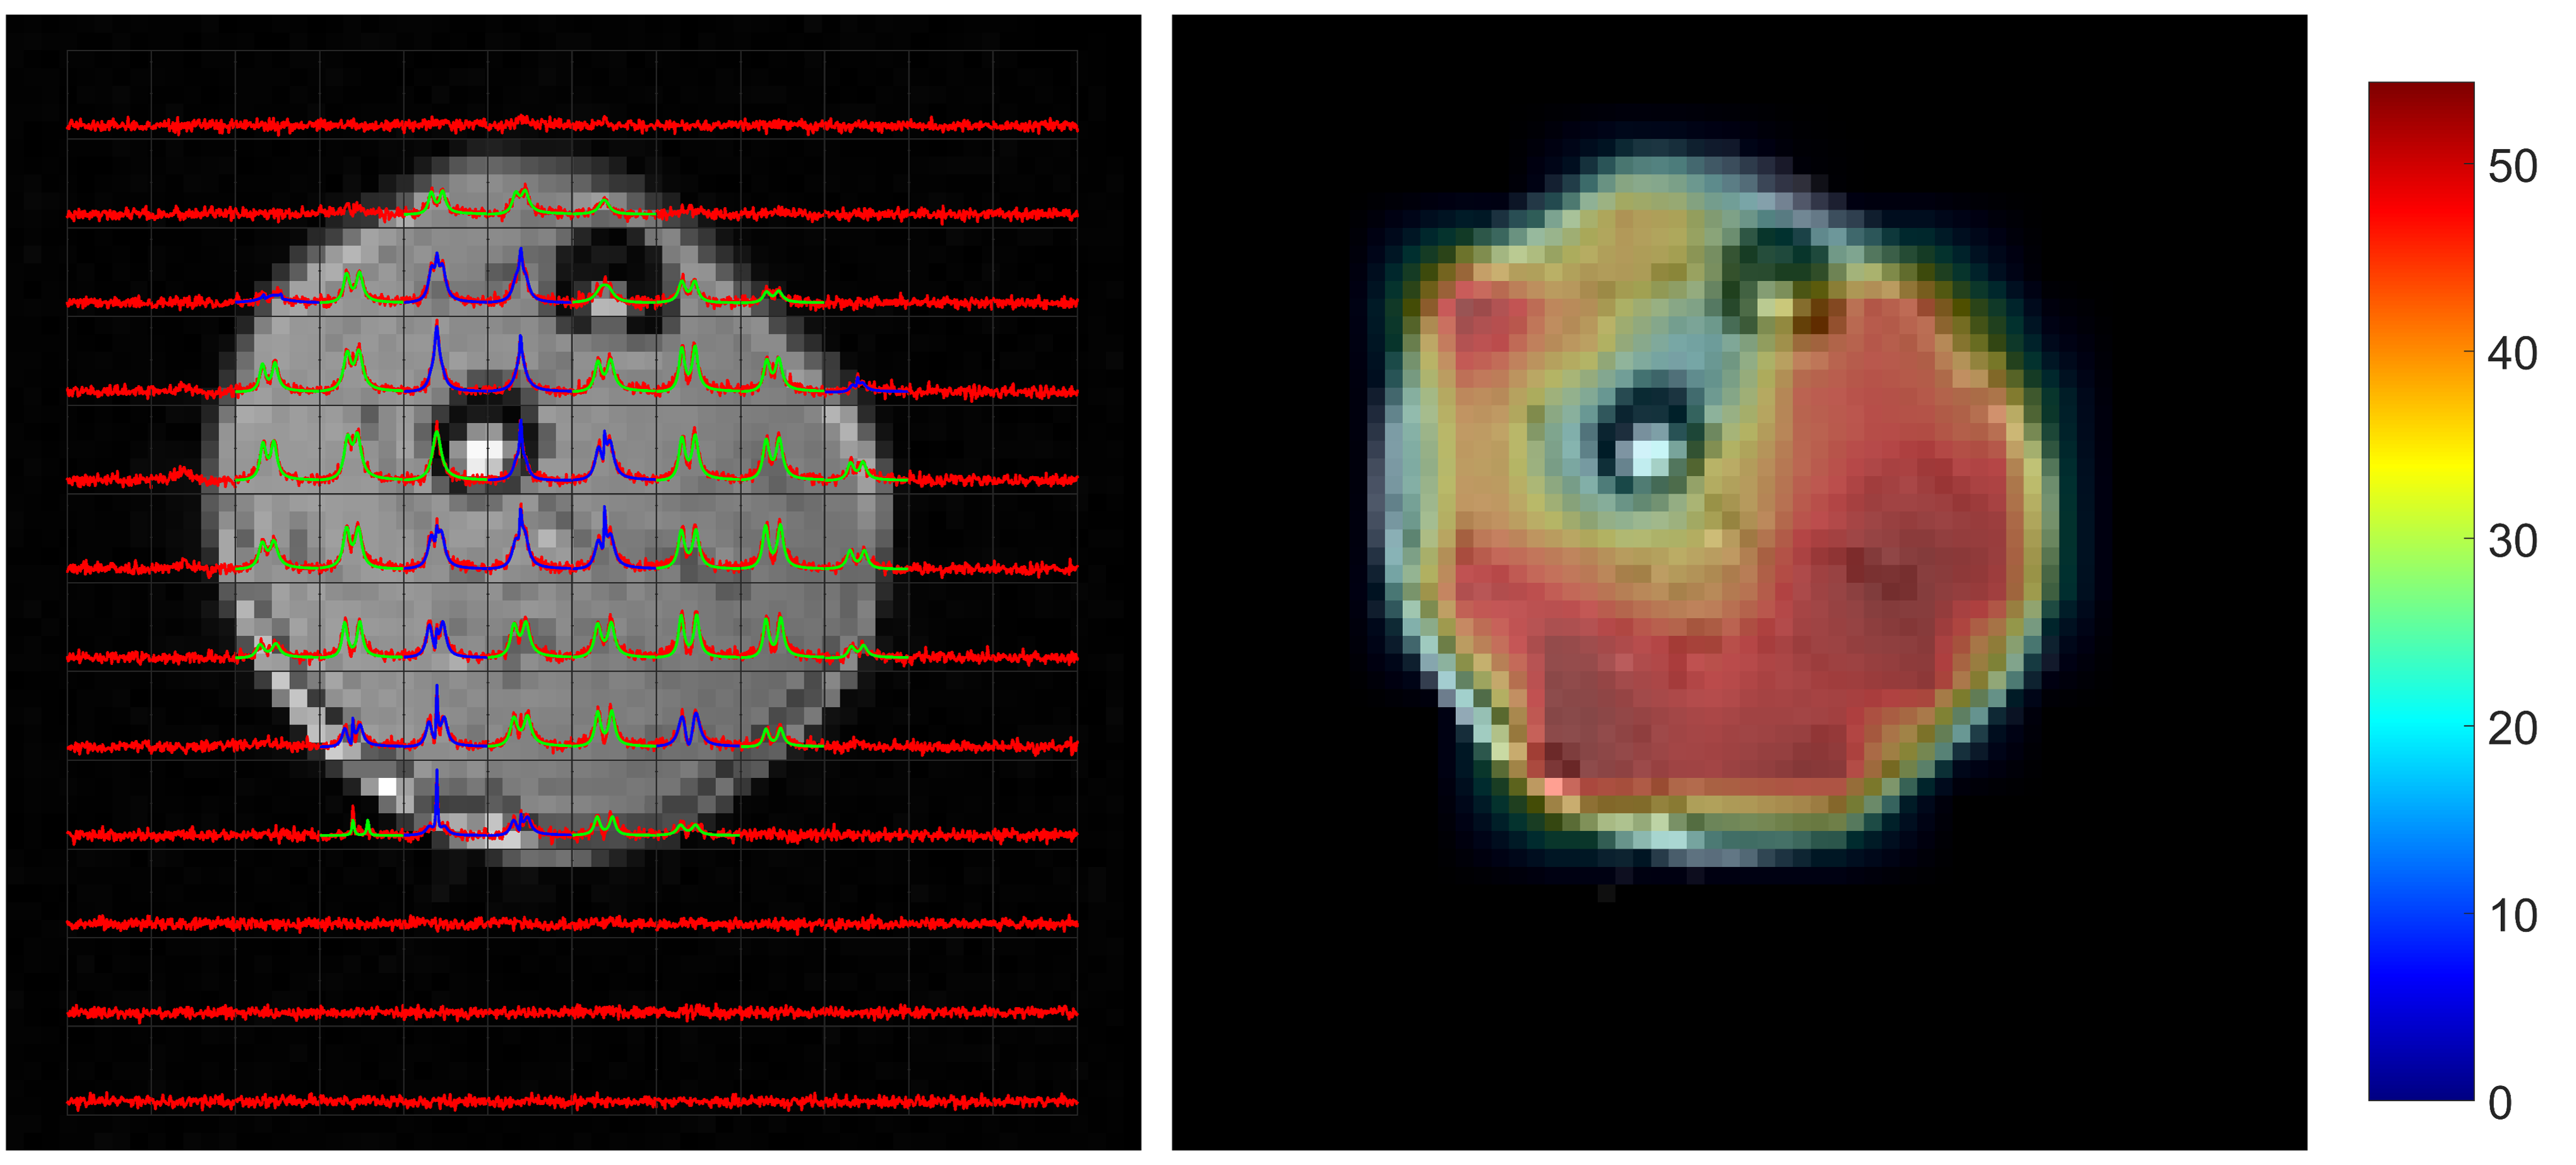
\includegraphics[width=1\textwidth]{Figures/Quad/Arm_A.png}
    \caption{Left: CSI spectra (red) overlayed onto a $^1$H GE image from participant A's left arm at an angle of 0 ${\circ}$ to the B0 field of a single slice, with fits of two Lorentzian peaks (green) and three Lorentzian peaks (blue). Right: Interpolated map of quadrupolar frequency splitting's overlayed onto the same $^1$H GE image from participant A's left arm. }
    \label{fig:D2O:Arm_A}
\end{figure}

\begin{figure}
    \centering
    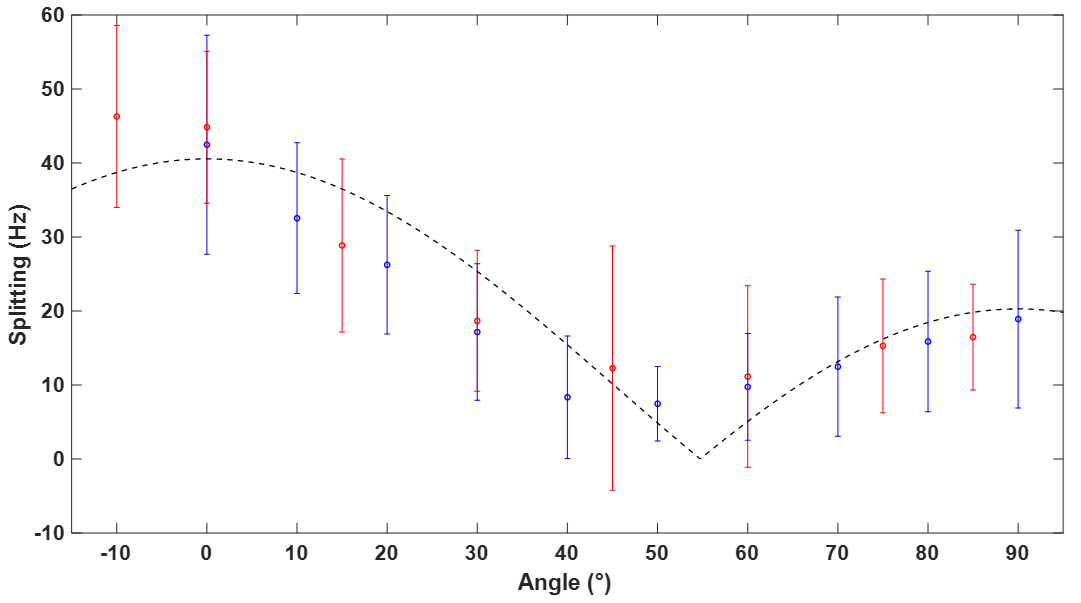
\includegraphics[width=1\textwidth]{Figures/Quad/Split_Angle_1.png}
    \caption{Graph Showing the variation of averaged quadrupolar frequency splittings of the arm against the angle to the B0 field they were positioned at, for partcipant A (blue) and B (red). Along with the fit (dotted black) of both participant's data to equation \ref{eqn:Quad:Angle}, the splitting magnitude of this fit is 38 $\pm$ 2 Hz.}
    \label{fig:D2O:Split_Angle}
\end{figure}

\subsection{DQF}

\section{Discussion}

\section{Conclusion}

% \printbibliography % Comment out main doc

\end{document}